% !TEX root = main.tex

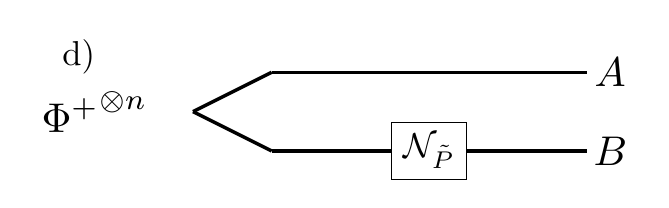
\begin{tikzpicture}
\node[scale=1.25] at (-1.45,0.7){d)};
\node[scale=1.5] at (-1.25,0){$\ket{\Phi^+}^{\otimes n}$};
\node[scale=1.5] at (5.3,1/2){$A$};
\node[scale=1.5] at (5.3,-1/2){$B$};
\draw[line width=1.25] (0,0) -- (1,1/2);
\draw[line width=1.25] (5,1/2) -- (1,1/2);
\draw[line width=1.25] (0,0) -- (1,-1/2);
\draw[line width=1.25] (5,-1/2) -- (1,-1/2);
\node[draw, scale=1.25, fill=white] at (3,-1/2){$\mathcal{N}_{\tilde{P}}$};
\end{tikzpicture}